\documentclass[12pt,a4paper]{article}
\usepackage[utf8]{inputenc}
\usepackage[czech]{babel}
\usepackage[T1]{fontenc}
\usepackage{amsmath}
\usepackage{amsfonts}
\usepackage{amssymb}
\usepackage{color,graphicx}
\usepackage{epstopdf}
\usepackage{indentfirst}
\setlength{\parindent}{4em} 
\author{Jakub Drápela}
\usepackage{fancyhdr}
\usepackage{siunitx}
\usepackage{pdflscape}
\usepackage[backend=bibtex,style=numeric,backref=true]{biblatex}
\definecolor{black}{gray}{0}
\usepackage[pdftex,unicode]{hyperref}
\hypersetup{colorlinks,pdfhighlight=/O,citecolor=black,
  filecolor=black,urlcolor=black,linkcolor=black,
  breaklinks=true,pdfpagemode=UseNone,plainpages=false,
}
\usepackage{filecontents}  % create "citations.bib" on-the-fly
\graphicspath{{./imgs/}}

%\fontfamily{phs}
%\selectfont

\begin{filecontents*}{businessPlan.bib}

@online{pict,
 author  = "The New York Times",
 title   = "The Amazon Echo",
 year    = "2015",
 urlseen = "03-17-16",
 url     = "http://static01.nyt.com/images/2015/06/25/business/GADGETWISE/GADGETWISE-master675.jpg",
}
\end{filecontents*}
\addbibresource{businessPlan.bib}

\begin{document}
\pagestyle{empty}

%%nastaveni pisma  
%\fontfamily{phv}
%\selectfont

	\begin{center}

\large

České vysoké učení technické v Praze\\
\medskip
Fakulta elektrotechnická\\[2cm]
{\LARGE\bfseries Household Intelligent Assistant}

\vfill
\begin{figure}[h!]
\begin{center}

\includegraphics[width = 5cm]{logo.pdf} 
\end{center}
\end{figure}
\vfill

\begin{tabular}{rl}

Autoři: & Jiří Burant \\
\noalign{\vspace{1mm}}
		& Jakub Drápela \\
		\noalign{\vspace{1mm}}
		& Martin Klučka\\
		\noalign{\vspace{1mm}}
		& Petr Kovář \\
		\noalign{\vspace{1mm}}
		& Jakub Konrád\\
		\noalign{\vspace{1mm}}
		& Pavel Trutman\\
\noalign{\vspace{2mm}}
Studijní obor: & Kybernetika a robotika \\
\noalign{\vspace{2mm}}
Datum vypracování: & \today\\
\end{tabular}

\end{center}

\newpage
\pagestyle{plain}     % zapne obyčejné číslování
\setcounter{page}{1}
%% zahlaví a zápatí
\addtolength{\voffset}{-3cm}
\addtolength{\headheight}{2cm}

\pagestyle{fancy}
\lhead{
\includegraphics[scale=0.12]{cvut_text.jpg}  }
\rhead{\textbf{Household Intelligent Assistant}}
%\rhead{\textit{\bfseries Burant,Drápela,Klučka,Kovář,Konrád,Trutman}}
\lfoot{}
\cfoot{\thepage}
\rfoot{}
\renewcommand{\headrulewidth}{0.4pt}

\section*{Úvod}
Cílem této zprávy je zhodnotit současný stav projektu \textit{Household Intelligent Assistant} a dosud dosažené výsledky, poskytnout detailní popis jeho jednotlivých součástí a stanovit časový plán, který povede k úspěšnému dokončení projektu v rámci naší časové dotace.
\section*{Aktuální stav projektu}
V současnosti existuje funkční prototyp osobního asistenta \textit{Phoenix}. Tento prototyp je umístěn ve virtuálním stroji na systému debian. Vytvořený prototyp dokáže úspěšne vnímat dotazy z oblasti počasí, vyhodnotit je a reagovat na ně. 

\subsection*{Popis prototypu}
Prototyp systému po spuštění vyčkává v režimu stand-by a čeká na aktivaci oslovením. Prototyp reaguje na oslovení klíčovým slovem (\textit{Phoenix}) a poté přepne do módu zaznamenávání dotazu. Prototyp zaznamená mluvený dotaz, převede jej do textové podoby, vyhodnotí jej a získá jeho význam. Dotaz je vyhodnocen a odpověď je získána pomocí webové aplikace třetí strany. Odpověď je poté převedena do textové podoby. Systém syntetizuje mluvenou odpověď ze získaného textu a odpoví uživateli.

Prototyp byl důkladně otestován členy projektu a během testování se objevily následující problémy: 
\begin{itemize}
	\item V neoptimálních zvukových podmínkách má systém problém s rozpoznáváním klíčového slova. Systém reaguje i pokud nebyl osloven klíčovým slovem.
	\item Prototyp má na některých zařízeních problém přijmout zvukový vstup.
	\item Systém se v některých případech po úspěšném zodpovězení dotazu nevrátí do stand-by režimu.
\end{itemize}


\subsection*{Stav projektu v rámci časového plánu}
Dle harmonogramu projektu se nacházíme ve fázi před druhým milníkem projektu, tedy vytvořením plně funkčního systému. Toto odpovídá skutečnému současnému stavu projektu. Už nyní existuje funkční verze systému, je tedy nutné pouze odstranit výše zmíněné problémy jsme připtaveni na vstup do finální fáze. Vytyčený plán se nám dosud podařilo dodržovat bez větších potíží. Věříme, že tomu tak bude i nadále a projekt bude ve stanoveném termínu úspěšně dokončen.



\section*{Detailní popis projektu}
Systém Phoenix je navržen modulárně tak, aby bylo možné jednoduše rozšiřovat a měnit jeho funkcoinalitu v závislosti na požadavcích uživatele. Celý systém je naimplementován v jazyce python a je rozdělen do několika základních modulů, které mezi sebou komunikují pomocí jádra aplikace (obrázek \ref*{fig:diagram api}). Následuje detailní popis řešení a funkce jádra a jednotlivých modulů:
\begin{figure}[ht]
	\begin{center}
		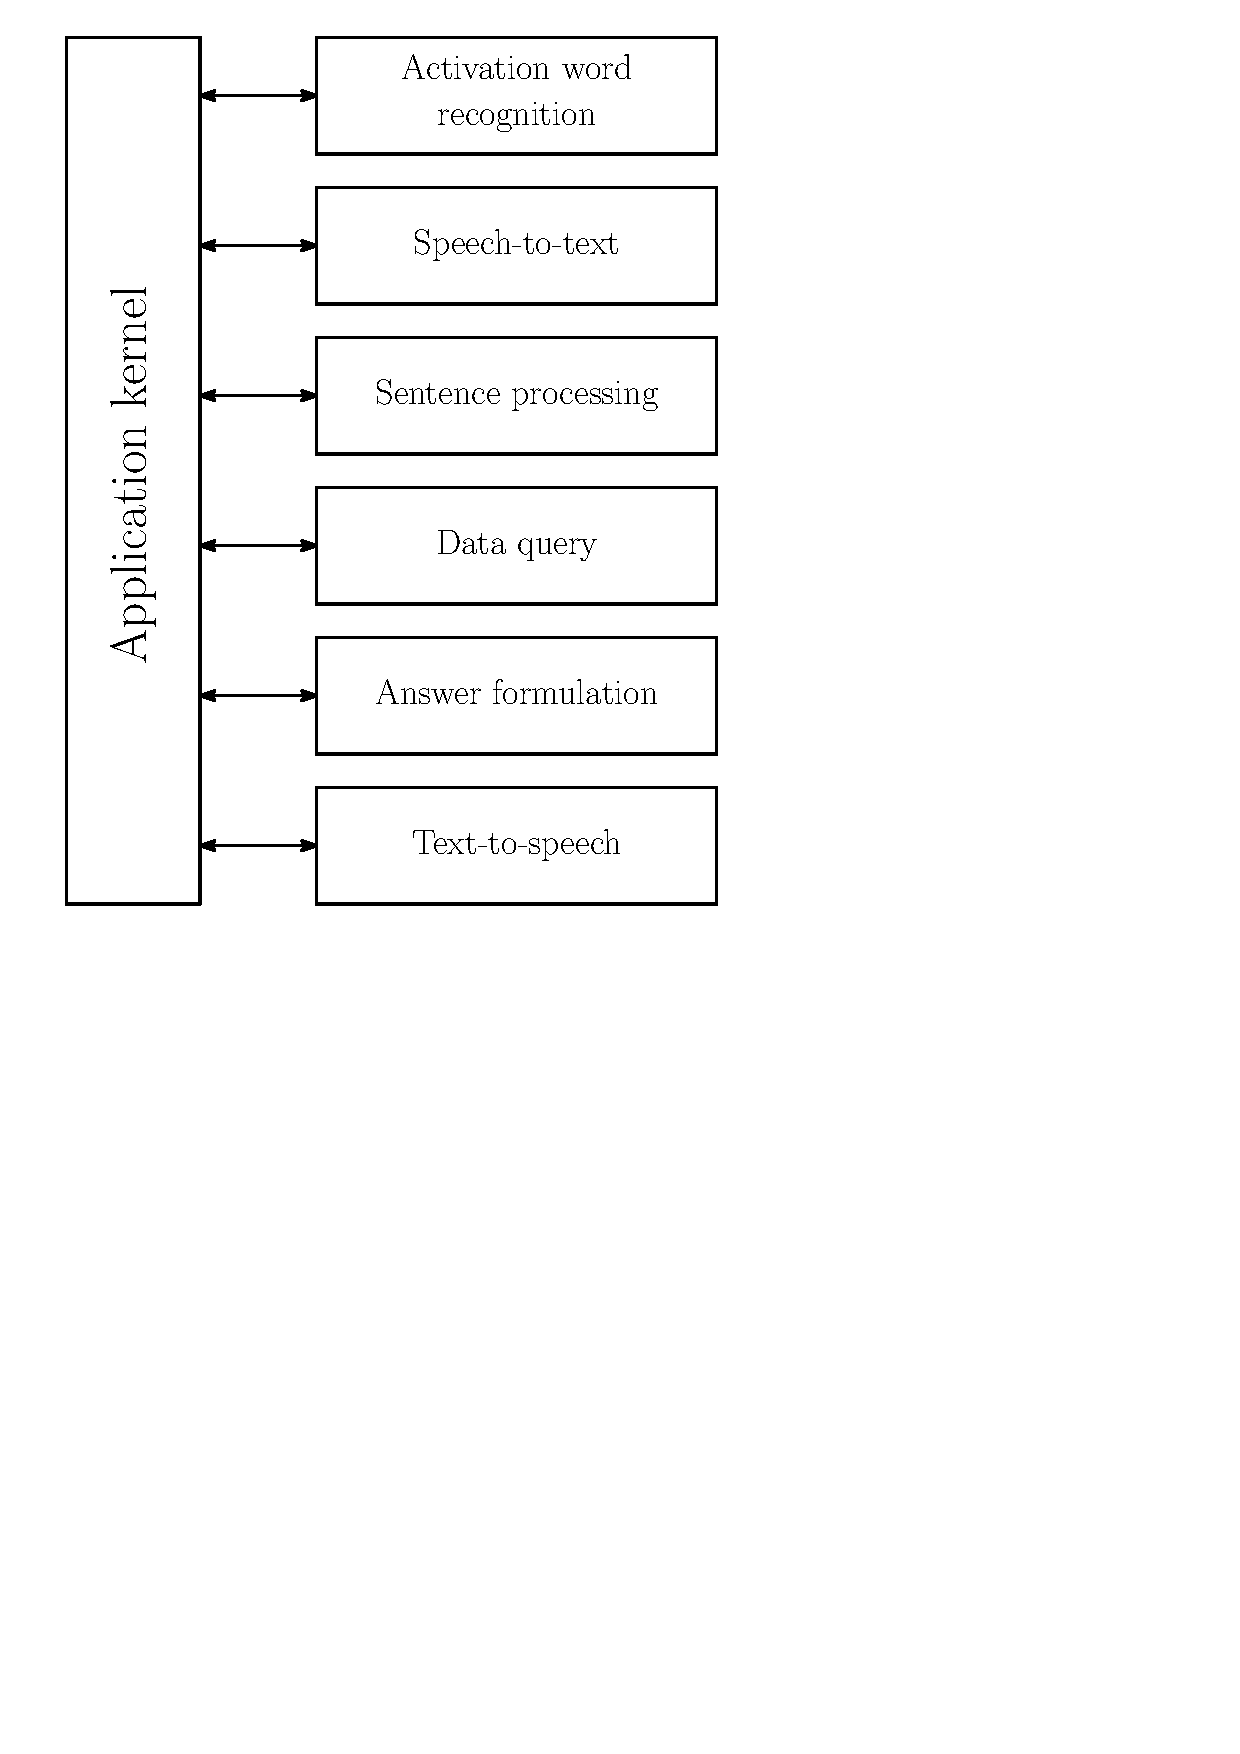
\includegraphics[height = 9cm]{blockDiagram.pdf}
		\caption{Blokový diagram řešení projektu Household Intelligent Assistant.}
		\label{fig:diagram api}
	\end{center}
\end{figure}


\subsection*{Activation word recognition a Speech-to-text}
S využitím knihovny \textit{PocketSphinx} byly v Pythonu implementovány mechanismy pro rozpoznávání klíčového slova (Keyword attention) a převod mluveného slova na text (Speech to Text). V obou případech bylo třeba řešit řadu minoritních problémů - za zmínku stojí například volba a implementace I/O knihovny pro práci s mikrofonním vstupem počítače. Oba výše zmíněné mechanismy jsme dále přepsali do samostatných modulů kompatibilních s jádrem aplikace (rozhranní \textit{Zero MQ}).

Modul pro detekci klíčového slova je od počátku nedílnou součástí navrženého řešení a tedy byl i jako jeden z prvních modulů propojen s jádrem. Za tři týdny testování jsme naměřili vysokou přesnost detekce, která je ale podmíněná vhodnou volbou parametrů pro daný mikrofon. Jako klíčové slovo slouží nadále slovo Phoenix s tím, že po blížícím se testování je možná jeho změna. V průběhu jsme se také potýkali s nestabilitou knihovny \textit{PyAudio}, která zajišťuje práci s mikrofonem. V současné době probíhá hledání a testování alternativních knihoven.


Modul pro převod mluveného na text slova je v současnosti implementován pomocí nástroje \textit{wit.ai}. Tuto implementaci v blízké době nahradí již připravený a samostatně otestovaný modul pro převod mluveného slova implementovaný pomocí \textit{PocketSphinx}. Od tohoto kroku si slibujeme rychlejší odezvu systému, neboť převod (na rozdíl od předchozího řešení) probíhá lokálně a offline. Přesnost převodu je opět na velmi dobré úrovni, kterou je případně možné dále vylepšit volbou gramatiky (Language Modelu) zaměřené na námi podporované domény. Podobně jako u modulu pro detekci klíčového slova, tak i zde se počítá se záměnou knihovny \textit{PyAudio} za některou z alternativ.
\subsection*{Sentence processing}
Modul pro parsování a zpracování dotazů byl naimplementován s využitím nástroje \textit{wit.ai}. Modul přijme dotaz v textové formě a pomocí pythnovskéhé knihovny se připojí k aplikaci \textit{wit.ai}, která pomocí námi vytvořené databáze rozparsuje dotaz a získá jeho význam (intent). 

Aplikaci \textit{wit.ai} jsme zvolili, protože s její pomocí se nám podařilo dosáhnout velmi dobrých výsledků při získávání výsledku dotazu a dále díky jednoduchým možnostem rozšíření její databáze. Databáze je v současné době zaměřena pouze na počasí avšak do konce projektu ji plánujeme rozšířit i o další oblasti.

Za zmínku stojí, že databáze se kterou aplikace \textit{wit.ai} pracuje je volně přístupná. Uživatel má možnost vytvořit si její kopii (fork) a modifikovat/doplnit ji tak, aby lépe vyhovovala jeho potřebám.

\subsection*{Data query a Answer formulation}
Modul, který obstarává vyhledávání informací a logiku, která má být vykonána na základě intentu se nazývá „querylogic“. Tento modul dostane od jádra jako vstup zpracovaný dotaz z \textit{wit.ai} a podle jeho významu vykoná žádané úkony a vyhledá potřebné informace. Následně vrátí zpět do jádra sestavenou odpověď ve formě textového řetězce.

V současné době je modul querylogic schopen obsluhovat základní dotazy z oblasti počasí, k tomu využívá internetové API \textit{forecast.io}, kterému posílá url request. Odpovědí je JSON objekt, ze kterého jsou vyčtena potřebná data, jako teplota, síla větru apod..
Dále tento modul používá knihovnu \textit{geopy}, která slouží k získání geografických souřadnic daného místa, pakliže ho tazatel specifikuje. 

Modul je schopen poskytnout informace o počasí na týden dopředu pro různá místa na zemi a je schopen poskytnout i historické údaje za posledních šedesát let. (Ty musí pro dané místo existovat).

Dále je rozpracován submodul obecné komunikace, který bude obstarávat některé běžné konverzační otázky, například:  “What is the time?“, “Tell me a joke.“, apod.
\subsection*{Text-to-speech}
Při realizaci tohoto modulu se jako největší problém ukázalo nalezení vhodné knihovny pro syntézu řeči. Z počátku jsme využívali knihovnu \textit{Pyttsx} v kombinaci s linuxovým ovladačen zvuku \textit{Espeak}. Zde se nám však nepodařilo dosáhnout požadované kvality syntetizované řeči a proto jsme se rozhodli od použití této knihovny odstoupit.

V současné době využívá náš modul syntetizátor řeči \textit{Mimic} od společnosti Mycroft. 
Tato knihovna má oproti předchozímu řešení výhodu jednoduchššího nastavení parametrů. S kvalitou syntetizovaného hlasu pomocí knihovny \textit{mimic} jsme spokojeni. Z řeči je sice patrné, že je počítačové povahy, avšak je srozumitelná a jedná se o výrazné zlepšení oproti předchozímu řešení.


\subsection*{Application kernel}
Jakmile byly vytvořeny všechny prototypy modulů, bylo třeba je zakomponovat do sebe tak, aby tvořily funkční aplikaci. K tomu slouží jádro aplikace, které s jednotlivými moduly komunikuje pomocí definovaného API. Jednotlivé moduly jsou jádrem spouštěny jako samostatné procesy, což dává velkou svobodu pro návrh a impementaci jednotlivých modulů, protože nejsou s jádrem vůbec svázány například vybraným programovacím jazykem.

K meziprocesové komunikaci mezi jádrem a moduly jsme použili knihovnu zeromq, která je rychlá a má jednoduché rozhraní pro většinu programovacích jazyků.

Skutečnost, že jednotlivé moduly komunikují s jádrem přes API, je výhodná i tom, že bylo-li potřeba některý modul nahradit za jiný, například z důvodu špatné funkčnosti použité knihovny, jen se vytvořil nový modul a v nastavení jádra aplikace stačilo jen změnit cestu k novému modulu. Žádné složité úpravy jádra tedy nebyly třeba. Tato velká modularita umožňuje případnému zájemci si kterýkoliv modul jednoduše upravit či vytvořit nový, aniž by musel podrobně zkoumat strukturu ostatních modulů nebo jádra aplikace.

\subsection*{Řešení pomocí virtuálního stroje}
Protože jednotlivé moduly použivají knihovny, jejichž instalace není snadná a liší se v závislosti na druhu operačního systému, vytvořili jsme virtuální stroj pro nástroj VirtualBox. Tento virtuální stroj běží na operačním systému Debian Jessie a obsahuje všechny nainstalované knihovny a balíčky potřebné pro běh naší aplikace, která je ve virtuálním stroji připravena ke spuštění. 

Vytvoření virtuálního stroje nám umožňilo vytvořit jednotné testovací rozhraní pro naši aplikaci a odbourali jsme tím mnoho problémů spojených s instalací potřebných knihoven na různých operačních systémech. Každý člen týmu tedy nemusel ztrácet čas zdlouhavou instalací všech knihoven na svůj počítač, ale stačilo mu jen si stáhnout obraz virtuálního stroje a ten spustit. Myšlenka virtuálního stroje nám také umožňuje jednoduše aplikaci nasílet dalším osobám mimo náš tým, které mohou aplikaci jednoduše testovat a nám tak poskytovat cennou zpětnou vazbu.

Pro sestavení virtuálního stroje používáme nástroj Vagrant, který velmi usnadňuje tvorbu a práci s virtuálními stroji. Pomocí Vagrantu si stáhneme již předinstalovaný operační systém, na který jednoduše nainstalujeme potřebné knihovny a naší aplikaci pomocí konfiguračního nástroje Ansible. Díky použití těchto dvou nástrojů můžeme jednoduše změnit operační systém na kterém aplikace běží přičemž nás to bude stát jen minimální úsilí. Takto tedy můžeme velmi efektivně testovat chování aplikace na různých operačních systémech.

Pokud chcete naší aplikaci vyzkoušet, můžete si stáhnout virtuální stoj na adrese [link dodám někdy později].

\section*{Neočekávané události}
V průběhu projektu došlo k následujícím neočekávaným událostem:
\begin{itemize}
	\item Změna rozhraní pythonovského modulu třetí strany \textit{pywit} pro použití aplikace \textit{wit.ai}
	
	Jak již bylo zmíněno, náš projekt využívá \textit{wit.ai} k parsování dotazu a získání jeho významu. Původně však \textit{wit.ai} zajišťoval také převod řeci na text. S vydáním nové verze \textit{pywit} byla tato funkcionalita omezena. V rámci našeho projektu bylo tedy nutno zareagovat a najít alternativní řešení. 
	
	Tento problém jsme přednesli na pravidelné týdení schůzce a po dohodě jsme přerozdelili plánovné úkoly na další týden tak aby došlo k vyřešení problému a zároveň nedošlo ke zpoždění projektu oproti harmonogramu.
	

\end{itemize}

\section*{Detailní plán do konce projektu}
Nyní se nacházíme ve druhé fázi projektu (viz harmonogram na obrázku \ref{fig:diagram gantt}), na jejímž konci bychom měli mít plně funkční systém. Tato fáze dle plánu končí 28. 4. 2016. Do tohoto data se tedy budeme věnovat především odstranění již zmíněných problémů prototypu, jmenovitě: odstranění problémů s nahráváním zvuku pomocí \textit{pyaudio}, zajištění spolehlivosti při rozpoznávání klíčového slova a zajištění přechodu systému do režimu stand-by po zodpovězení dotazu.

Po vyřešení těchto problémů a přechodu do finální verze projektu, která má probíhat od 29. 4. 2016 do 19. 5. 2016 nás čekají dva hlavní úkoly a to: 
\begin{itemize}
	\item Rozšíření funkcionality a přidání jednoduchých “obecných“ modulů pro zajištění větší flexibility systému (např.: time modul - sdělí uživateli čas, joke modul - řekne uživateli vtip z databáze, atd.).
	\item Důkladné testování systému. Systém bude podroben důkladnému testu a to i uživateli mimo skupinu vývojářů projektu tak, aby došlo k zachycení a opravení jeho případných bugů a nedostatků.
\end{itemize}

\begin{landscape}
~\vfill
\begin{figure}[ht]
	\begin{center}
	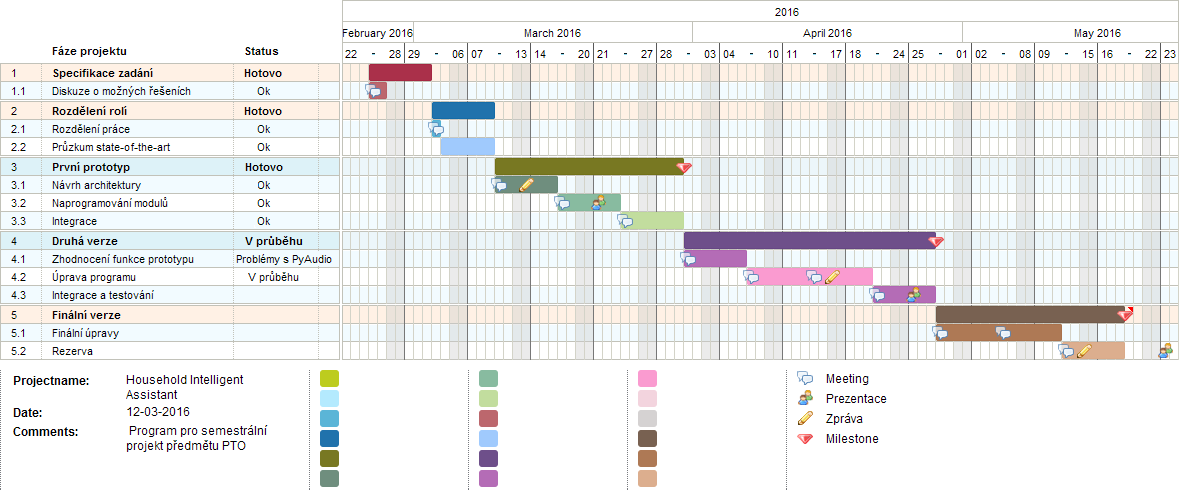
\includegraphics[height = 0.6\textheight ]{PTO-Gantt.png}
	\caption{Harmonogram projektu graficky znázorněn formou Ganttova diagramu s klíčovými milníky.}
	\label{fig:diagram gantt}
	\end{center}
\end{figure}
\vfill
\end{landscape}

\end{document}
